\chapter{The Bayesian Method}
\label{sec:inference_methodology}

\section{Income Homophily}
\label{subsec:income_homophily}

The main contribution of this work is the estimation of the income of the telco users for which we lack banking data, but have bank clients in their neighborhood of the network graph. To show the feasibility of this task, we first show the existence of a strong income homophily in the telco graph as is evidenced in \Cref{fig:homophily_heatmap}.

\begin{figure}
\centering
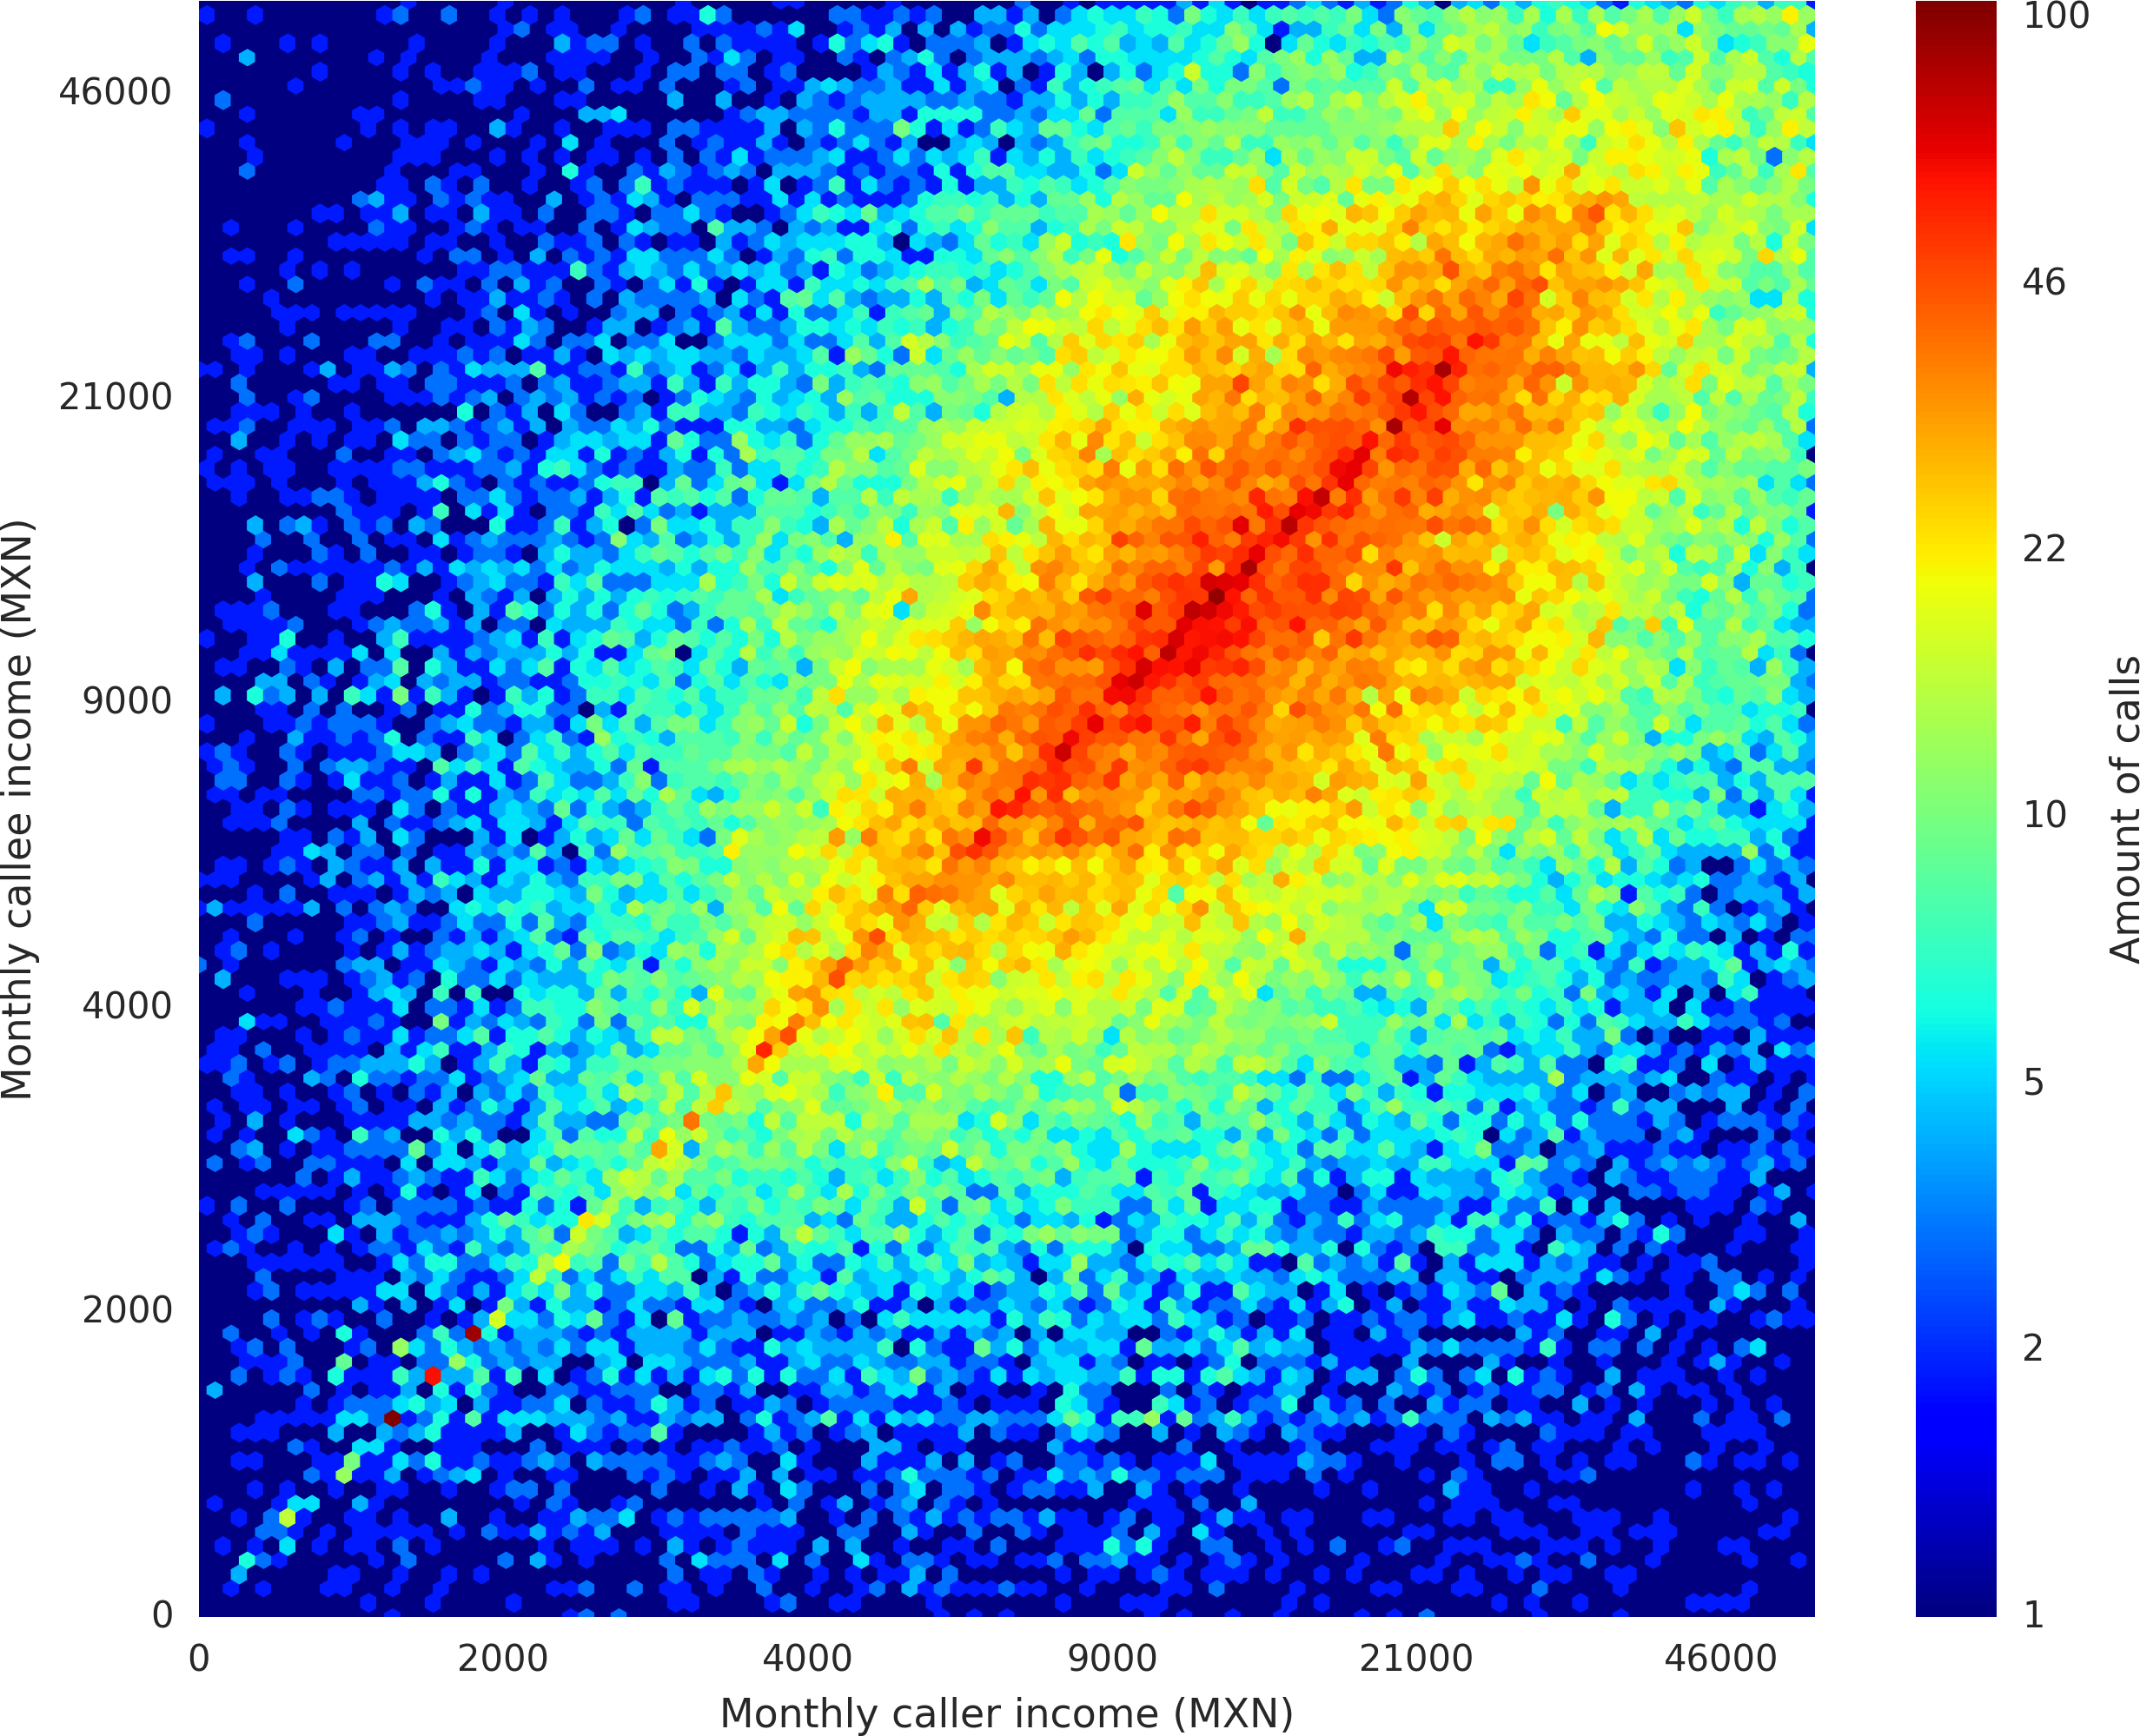
\includegraphics[width=\textwidth]{figures/Homophily_income_origin_target_1/Homophily_income_origin_target_1.png}
\caption{Heatmap showing the number of calls between users, according to their monthly income. There is a higher probability that the callee and the caller have similar income levels.}
\label{fig:homophily_heatmap}
\end{figure}

For each pair $\left\{ \left< p_o, p_d \right> \mid p \in P \right\}$, the X coordinate is defined as the set of incomes for callers, while the Y coordinate is the set of incomes for callees. According to what we can observe in \Cref{fig:homophily_heatmap}, there should be a significant correlation between $X$ and $Y$. Given the broad non-Gaussian distribution of the income's values, we choose to use a rank-based measure of correlation which is robust to outliers.

Namely, the \textit{Spearman's rank correlation}, as defined in defined in \Cref{spearman}, is computed to test the statistical dependence of sets of incomes of callers and callees. Applying this formula to the data gives a correlation coefficient of $\mathbf{r_s = 0.474}$.

The result was compared with a randomized null hypothesis, where links between users are selected randomly disregarding income data, obtaining a $p\text{-value}$ of $p < 10^{-6}$. These values for $r_s$ and $p$ show a strong indication of income homophily among users in our communication graph. This observation is consistent with the results reported in other investigation of similar data, namely~\cite{leo2015socioeconomic}.

We can take advantage of this homophily to propagate income information to the rest of our graph $P$, where the income of the complete set of users is unknown.

\section{Prediction Algorithm}
\label{subsec:prediction_algorithm}

\subsection{Discrimination by Wealth}
\label{subsec:discrimination_by_wealth}

The main objective of this research is to identify users with higher income. To make the task simpler and more efficient, the actual income values as described in \Cref{subsec:bank_source} are forfeited and instead the customers are separated into distinct groups: $H_1$, containing customers whose income is lower or equal than the median, and $H_2$, containing users whose income is higher than this value. From now on, these will be referred as \emph{Low Income} and \emph{High Income} users respectively.

The median value in the dataset, after accounting for outliers as explained in \Cref{subsec:outlier_filtering}, is of exactly \textbf{6300 MXN}. This way, we can define the two groups as in \Cref{eq:h}.

\begin{equation}
\label{eq:h}
\begin{gathered}
H_1 \cup H_2 = S \\
\left( \forall h \in H_1 \right) h_s \leq 6300 \\
\left( \forall h \in H_2 \right) h_s > 6300
\end{gathered}
\end{equation}

\subsection{Feature Accumulation}
\label{subsec:feature_accumulation}

Given the \emph{Social Graph} $G = \left< V, E \right>$, as defined in \Cref{sec:dataset}, contains information about the \emph{Calls}, \emph{SMS}, and \emph{Total Time} of each link between two users. These can be accumulated for each user, along with its \emph{Degree}, to produce the \emph{User Data}, which is used for another evaluation in \Cref{subsec:user_data}.

Another possible way to accumulate these values is discriminating them by the category to which the other endpoint belong. That is, for every edge feature $F$ and for the \emph{Degree}, it's possible to define two features $F_{\low}$ and $F_{\high}$ that only accumulate features from edges whose other endpoint is a user with \emph{Low Income} or \emph{High Income}, respectively. This approach is formalized in \Cref{eq:bayesian_accum}.

\begin{equation}
\label{eq:bayesian_accum}
\begin{gathered}
\begin{aligned}
& \calls^{\low}_v = \sum_{\substack{e \in E \\ e_d = v \\ e_o \in H_1}}{e_c} + \sum_{\substack{e \in E \\ e_o = v \\ e_d \in H_1}}{e_c}
& \calls^{\high}_v = \sum_{\substack{e \in E \\ e_d = v \\ e_o \in H_2}}{e_c} + \sum_{\substack{e \in E \\ e_o = v \\ e_d \in H_2}}{e_c} \\
& \etime^{\low}_v = \sum_{\substack{e \in E \\ e_d = v \\ e_o \in H_1}}{e_t} + \sum_{\substack{e \in E \\ e_o = v \\ e_d \in H_1}}{e_t}
& \etime^{\high}_v = \sum_{\substack{e \in E \\ e_d = v \\ e_o \in H_2}}{e_t} + \sum_{\substack{e \in E \\ e_o = v \\ e_d \in H_2}}{e_t} \\
& \sms^{\low}_v = \sum_{\substack{e \in E \\ e_d = v \\ e_o \in H_1}}{e_s} + \sum_{\substack{e \in E \\ e_o = v \\ e_d \in H_1}}{e_s}
& \sms^{\high}_v = \sum_{\substack{e \in E \\ e_d = v \\ e_o \in H_2}}{e_s} + \sum_{\substack{e \in E \\ e_o = v \\ e_d \in H_2}}{e_s}
\end{aligned} \\
\begin{aligned}
\contacts^{\low }_v &= c^{\low}_v &= &\left| \left\{ e \in E \; \middle| \begin{aligned} &e_o = v &\land &\quad e_d \in H_1 \\ &&\lor & \\ &e_d = v &\land &\quad e_o \in H_1 \end{aligned} \right\} \right| \\
\contacts^{\high}_v &= c^{\high}_v &= &\left| \left\{ e \in E \; \middle| \begin{aligned} &e_o = v &\land &\quad e_d \in H_2 \\ &&\lor & \\ &e_d = v &\land &\quad e_o \in H_2 \end{aligned} \right\} \right|
\end{aligned}
\end{gathered}
\end{equation}

\subsection{Uncertainty}
\label{subsec:uncertainty}

One important thing to note is that the only nodes accumulated in \Cref{eq:bayesian_accum} for some node $v \in V$ are the neighbouring ones that belong to $S$. \Cref{eq:subset_neighbours} indicates how to build the subset $D \subseteq S$ of bank users who also have a neughbour in the \emph{Social Graph} $G$ which is also part of the bank.

\begin{equation}
\label{eq:subset_neighbours}
\begin{gathered}
E^D = \left\{ e \in E \mid e_o \in S \land e_d \in S \right\} \\
D = E^D_o \cup E^D_d
\end{gathered}
\end{equation}

$D$ is defined as a subset of $S$, instead of one of $V$, because we cannot analyze the performance of a predictor on telco users who aren't part of the bank.

There is an additional level of uncertainty: while the data contains information about calls, and the inference assumes that callee and caller know each other, there is simply no information about the socioeconomic level of acquaintances who don't share phone calls. However, the more calls a user names, and the more people it calls, the more \emph{Certain} we can be that the algorithm in this section is correct.

\subsection{Modelling Users --- Frequentist Approach}
\label{subsec:modelling_users_frequentist}

The final objective of this thesis is to detect \emph{High Income} users in a dataset by just knowing their calls using the hypothesis, described in Section~\ref{subsec:income_homophily}, that a user will mostly call people from his same income category. For this, some calculated will be made on the low and high calculations for some property $\varpi$\footnotemark{}, which is one of the values defined in Equation~\ref{eq:property}. Part of the performance calculations in Section~\ref{sec:results} will imply finding the $\varpi$ which maximizes some score.

\footnotetext{$\varpi$ is a variant of the Greek letter $\pi$, which represents a \textbf{P}roperty.}

\begin{equation}
\label{eq:property}
\varpi \in \left\{ \calls, \etime, \sms, \contacts \right\}
\end{equation}

As it was discussed in Section~\ref{subsec:uncertainty}, even having that data it's impossible to have complete information about a user's relationships. However, it's possible to create a \emph{Model} where we can predict the rate of \emph{High Income} to \emph{Low Income} contacts a user has, and with that data the Probability $p_v$ that this user $v \in V \setminus B$ is a \emph{High Income} user.

The naïve way of solving this problem would be to assign this probability using only the current data, as in Equation~\ref{eq:naive_p}. However, this fails to account for the \emph{Certainty} that a user belongs to some category, which can be exemplified in scenarios where the probability of a user with only 1 \emph{High Income} contact being \emph{High Income} is slightly higher than one for another user with 100 \emph{High Income} contacts and 1 \emph{Low Income} contact.

\begin{equation}
\label{eq:naive_p}
p_v = P \left( v \in H_2 \right) = \frac{\varpi^{\high}_v}{\varpi^{\high}_v + \varpi^{\low}_v}
\end{equation}

\subsection{Modelling Users --- Bayesian Approach}
\label{subsec:modelling_users}

This section uses a variant of the \emph{Beta-Binomial Model} presented in Section~\ref{subsec:betabin}.

For each user $v \in V \setminus B$ we define a \emph{Beta Distribution} $\Betadist_v$ which can define the probability of $p_v$ falling between two numbers. This approach is formalized in Equation~\ref{eq:beta}.

\begin{equation}
\label{eq:beta}
	\Betasim_v \sim \Betadist_v \left( \varpi^{\high}_v + 1, \varpi^{\low}_v + 1 \right)
\end{equation}

The previous equation allows us to define a formula for the probability of each users $p_v$, as shown in Equation~\ref{eq:betaleq}.

\begin{equation}
\label{eq:betaleq}
	P \left( \Betasim_v \leq x \right) = \frac{1}{\Beta \left( \varpi^{\high}_v + 1, \varpi^{\low}_v + 1 \right)} \cdot \int_0^x {t^{\varpi^{\high}_v} {\left( 1 - t \right)}^{\varpi^{\low}_v} dt}
\end{equation}

Here it's also possible to assign the probability depending on the \emph{Mean} or the \emph{Mode} of the distribution. However, that would also fail to account for the \emph{Certainty} of the numbers, which is the disadvantage discussed in the method defined in Section~\ref{subsec:modelling_users_frequentist}.

Instead, given the definition of an arbitrary $\Theta \in \left[ 0, 1 \right]$, it's possible to use the formula presented in Section~\ref{subsec:beta_ppf} to define a suitable $p_v$, as shown in Equation~\ref{eq:beta_theta_ppf}.

\begin{equation}
\label{eq:beta_theta_ppf}
\begin{aligned}
p_v &= Q \left (\Theta \right) \\
&= \inf \left\{ x \in \left[ 0, 1 \right] \mid \Theta \leq F(x) \right\}
\end{aligned}
\end{equation}

This probability represents the \emph{Posterior Probability} of $p_v$ given the data. To adjust the prediction, the method compares the value for each user with the rest and assumes that, if $p_v > p_u$ for two users $v$ and $u$, then $v$ has a higher probability of being wealthy.

Since we don't have any prior information about a good value of $\Theta$, we initially take a value from \emph{Jeffrey's Prior}. This distribution, which was defined by Harold Jeffreys in 1946~\cite{jeffreys46}, is a completely uninformative prior distribution for a parameter that makes it possible to parametrize prior ignorance about values in a Bernoulli model.

The \emph{Probability Density Function} of the prior for a parameter $\gamma$ is presented in Equation~\ref{eq:jeffreys}. It's important to note that this is the same PDF than in the one for a \emph{Beta Distribution} with parameters $\alpha = \sfrac{1}{2}, \beta = \sfrac{1}{2}$.

\begin{equation}
\label{eq:jeffreys}
	P \left( \Theta = \gamma \right) \propto \frac{1}{\sqrt{\gamma \left( 1 - \gamma \right)}}
\end{equation}

\subsection{Categorizing Users}

In the previous section the probability of belonging of being a \emph{High Income} user $p_v$ was defined for every $v \in V \setminus B$. While this value alone doesn't give any information about whether user $v$ belongs which category, it does tell that his category will be higher or equal than users with a lower probability. This approach is formalized in Equation~\ref{eq:pv_minus}.

\begin{equation}
\label{eq:pv_minus}
\begin{gathered}
	\left( \forall u, w \in V \setminus B \right) \\
	\begin{aligned}
		p_u > p_w \land u \in H_1 &\implies w \in H_1 \\
		p_u < p_w \land u \in H_2 &\implies w \in H_2 \\
		p_u = p_w \implies ( u \in H_1 &\iff w \in H_1 )
	\end{aligned}
\end{gathered}
\end{equation}

Thanks to this approach we can define some limit, $\tau$, and categorize each user $v \in V \setminus B$ as either category depending on the magnitude of $p_v$ compared to $\tau$, as in Equation~\ref{eq:pv_tau}.

\begin{equation}
\label{eq:pv_tau}
\begin{aligned}
p_v \leq \tau &\implies v \in H_1 \\
p_v > \tau &\implies v \in H_2
\end{aligned}
\end{equation}

\section{Performance Evaluation}
\label{subsec:performance_evaluation}

It's easy to evaluate the performance by calculating $p_v$ for all $v \in B$, which allows us to know whether each value is a \emph{True~Positive}, a \emph{False~Positive}, a \emph{False~Negative}, or a \emph{True~Negative}, and collecting any of the metrics described in Section~\ref{subsec:mlmetrics}.

One advantage of this method is that it's possible to evaluate the method by calculating the \emph{Area Under the Curve} without having to specify a particular $tau$, since this follows the necessary pattern defined in Section~\ref{subsec:auc}. This way it's possible to select the best $\varpi$ without having to select the respective $\tau$.

Additionally, after defining a $\varpi$, it's easy to select a $\tau$ so that the final \emph{Accuracy} is maximized.

\section{Bayesian Graphical Model}
\label{subsec:bayesiangm}

An alternative way of seeing this problem is through a \emph{Bayesian Graphical Model}, which are explained with more detail in~\cite{wagenmakerslee}.

In the model, shown in Figure~\ref{fig:bayesnetwork}, instead of defining a Beta distribution $\Betasim_v \sim \Betadist(\varpi^{\high}_v + 1, \varpi^{\low}_v + 1)$ for every user $v$, the problem is defined as a \emph{Binomial Distribution} which should have the respective parameters.

For simplicity, other two new categorical variables are defined for this model for each user $v$: $\varkappa_v$, which is 1 if and only if $v$ is part of the high category of income, and $\hat{\varkappa}_v$, which is 1 if and only if $v$ is predicted to be of the high category of income.

\begin{figure}
\centering
\begin{minipage}[l]{0.45\textwidth}
\begin{tikzpicture}
	\node[obsDisc] (n) {$n_v$};
	\node[obsDisc, below = 0.75 of n] (k) {$k_v$};
	\node[latentCont, below = 0.75 of k] (pi) {$\pi_v$};
	\node[detCont, below = 0.75 of pi] (p) {$p_v$};
	\node[latentCont, left = 1 of p] (theta) {$\Theta$};
	\node[detDisc, below = 0.75 of p] (hkappa) {$\hat{\varkappa}_v$};
	\node[obsDisc, below = 0.75 of hkappa] (kappa) {$\varkappa_v$};
	\node[detCont, right = 1 of p] (tau) {$\tau$};

	\edge {n} {k};
	\edge {pi} {k};
	\edge {pi} {p};
	\edge {theta} {p};
	\edge {p} {tau};
	\edge {p} {hkappa};
	\edge {tau} {hkappa};

	\draw[->, rounded corners = 10pt] (kappa) -| (tau);

	\plate [xshift = 1.1em] {} {(n) (k) (pi) (p) (hkappa) (kappa)} {$v \in V \cap B$};
\end{tikzpicture}
\end{minipage}
\begin{minipage}[r]{0.4\textwidth}
\begin{align*}
	n_v &= \varpi^{\high}_v + \varpi^{\low}_v \\
	k_v &= \varpi^{\high}_v \\
	\varkappa_v &= \begin{cases} 0 \ \text{if} \ v \in H_1 \\ 1 \ \text{if} \ v \in H_2 \end{cases} \\[1em]
	\pi_v &\sim \Binom \left( n, v \right) \\
	\Theta &\sim \Betadist(\sfrac{1}{2}, \sfrac{1}{2}) \\
	p_v &= \inf_{x \in \left[ 0, 1 \right]} \left\{ \Theta \leq P \left( \pi_v \leq x \right) \right\} \\
	\tau &= \argmax_{t \in \left[ 0, 1 \right]} \left| \bigl\{ \vspace{4em} v \in V \cap B \mid p_v \geq t \iff k_v \bigr\} \right| \\[1em]
	\hat{\varkappa}_v &= \begin{cases} 0 \ \text{if} \ p_v < \tau \\ 1 \ \text{if} \ p_v \geq \tau \end{cases}
\end{align*}
\end{minipage}
\caption{A Bayesian Graphical Model representing an interesting alternative approach to the problem, using a \emph{Binomial Distribution} instead of a \emph{Beta Distribution}. If this model was applied with a program such as \texttt{Jags}, the results would be the same.}
\label{fig:bayesnetwork}
\end{figure}

